\documentclass[a4paper, 12pt]{report}
\usepackage[utf8]{inputenc}
\usepackage[swedish,british]{babel}
\usepackage{graphicx}
\usepackage{fancyhdr}
\usepackage{float}
\usepackage{placeins}

\usepackage{listings}
\usepackage{glossaries}
\pagestyle{fancy}
\begin{document}

\graphicspath{{./images/}}
\title{Smarter Scrabble - strategies and their impact}
\date{Course: DD143X \\ Supervisor: Johan Boye \\ Kungliga Tekniska Högskolan \\ CSC \\ March 7, 2012}
\author{Frej Connolly \\ Götgatan 78 13TR LÄG1302 \\ 118 30 Stockholm \\ SWEDEN \\ +46(0)73-963 41 90 \\ connolly@kth.se \\
        \and Diana Gren \\ Sköldgatan 8 2TR \\ 118 63 Stockholm \\ SWEDEN \\ +46(0)70-467 47 20 \\ dianagr@kth.se}

\maketitle
\begin{abstract}
Scrabble is a well known board game that lets its players face many problems while playing. To become a successful Scrabble player, one can focus on learning certain things and instantly advance. This study investigates parts of the game one could choose to learn in order to become a better player. The aim is to evaluate different strategies in order to see what impact they have on a game. Three agents with one naive strategy is played against each other; place words with high score, always hit bonus squares if possible, and keep a good balance between consonants and vowels on the rack. 

The results show that always hitting bonus squares is a rewarding strategy, as the agent following that strategy won over the other two. They also show that there is a slightly higher chance of winning if being the player starting the game. Conclusions made from the results are that even though one probably would prefer placing a long word with higher score, it is not always the best move to choose. Also, to learn few lettered words, and many word extensions is rewarding when following the strategy with hitting bonus squares.
\end{abstract}

\selectlanguage{swedish}
\begin{abstract}
Scrabble 
\end{abstract}
\selectlanguage{british}

\subsubsection{Statement of collaboration}
Since the project was executed by two people, we are required to specify which person contributed with  which parts. 

The implementation was mostly made together, though some distributions were made to make it more efficient:
\begin{itemize}
\item{Frej}: Dictionary representation
\item{Diana}: Word generation
\end{itemize}

As of the report, the list below is a rough indication of how the work was distributed a part from all that was made together.

\begin{itemize}
\item{Frej}: Sections \ref{sec:rules}, \ref{dic-rep}, \ref{sec:bonusHigh}
\item{Diana}: Sections \ref{sec:agents}, \ref{sec:highBalance}, \ref{sec:balanceBonus}
\end{itemize}

\tableofcontents





\chapter{Introduction}
Scrabble is an old classic board game, with game rules that are not very complicated. However, it is extremely difficult to be a great player \cite{perfectgame}. Compared to other classic board games, such as Chess, there are more factors to take into consideration when making a move in Scrabble. 

Apart from anagramming and generating words, there are other crucial decisions to make. A player would probably find several legal moves in one round, and then would have to decide which one to place. Choosing the move that generates the highest score is not always the ideal way to go. It could be that making such a move would create a situation in the next round where nothing could be done, or let the opponent score high.

Making the choice of which move to use include many factors, and there are several different techniques and strategies one can follow to make the decision easier. Hitting the bonus squares can generate an extremely high score, hence one strategy is to try to always hit the bonus squares and prevent the opponent from doing the same. Another way of being successful is to prioritize using letters with high score, since they would not only generate a high total score to the player, but could also create difficult situations in the future if not used as soon as possible.

There are several more possible strategies one can follow, and this study aims to investigate three of them and try to establish which one is the most rewarding.

\section{Problem statement}
Which strategies have the most impact on a game? How do the strategies perform against each other, and which is the most successful one?

Scrabble requires the players to have a good vocabulary and to become a successful player, some knowledge about how many tiles of each letter is available is preferable. 

When playing, the ability to keep a good balance between consonants and vowels on the rack can benefit future moves. Destroying bonus possibilities for the opponent, and at the same time score them oneself is a crucial skill, and experts are probably aware of which tiles have been placed, and those that remain, allowing them to anticipate the future sequence of events. This study will test three agents with different strategies, and evaluate which strategy would be more rewarding to focus on when learning Scrabble.


\section {Terminology}
\label{sec:terminology}

\begin{description}
\item{\bf{Anchor square}}: Vacant board square adjacent to a placed tile.

\item{\bf{Bag}} Tiles that have not been drawn by players.

\item{\bf{BOR}}: Balance on rack player.

\item{\bf{BS}}: Bonus square player.

\item{\bf{Cross check set}}: Set of possible letters on an anchor square with regard to adjacent word going vertical from named square.

\item{\bf{DAWG}}: Directed acyclic word graph.

\item{\bf{HSW}}: High score word player.

\item{\bf{Rack}} Tiles on a player's hand. 

\end{description}







\chapter{Background}

\section{Scrabble game rules}
\label{sec:rules}
Scrabble is word game for two to four players. They are given a set of letter tiles and the game objective is to form words to place onto a board of squares \cite{ABSP} \cite{NASPA} \cite{forbund}.

\begin{figure}[h]
\centering
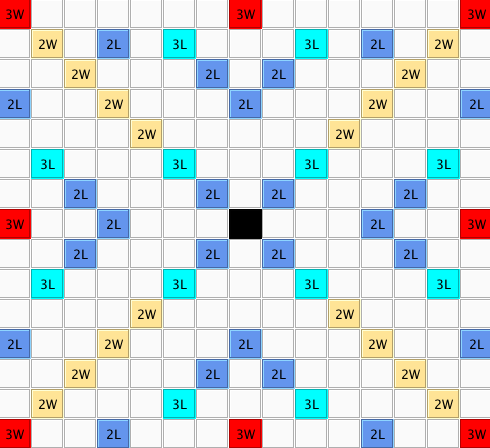
\includegraphics[scale=0.55]{board}
\caption {Game board. 15x15 square board with bonus squares.}
\label{fig:game-board}
\end{figure}

\subsubsection{Game components}
Scrabble consists of 

\begin{itemize}
\item a 15x15 board with bonus squares and the center marked out. See figure \ref{fig:game-board}.
\item a set of letter tiles
\end{itemize}

The players are given 5-8 tiles each to keep on their \emph{rack}. Each letter reward points. Letters that are frequent in the language give lower score, and letters that exist in fewer words give higher score. The following list shows the letter scores and the number of occurances of each tile in the bag \cite{letterpoints}.

\begin{itemize}
\label{letter+table}
	\item{\emph{1 point}} \textbf{A}x8, \textbf{D}x5, \textbf{E}x7, \textbf{I}x5, \textbf{L}x5, \textbf{N}x6, \textbf{R}x8, \textbf{S}x8, \textbf{T}x8
	\item{\emph{2 points}} \textbf{G}x3, \textbf{H}x2, \textbf{K}x3, \textbf{M}x3, \textbf{O}x5
	\item{\emph{3 points}} \textbf{F}x2, \textbf{V}x2, \textbf{Å}x2
	\item{\emph{4 points}} \textbf{B}x2, \textbf{P}x2, \textbf{U}x3, \textbf{Ä}x2, \textbf{Ö}x2
	\item{\emph{7 points}} \textbf{J}x1, \textbf{Y}x1
	\item{\emph{8 points}} \textbf{C}x1, \textbf{X}x1
	\item{\emph{10 points}} \textbf{Z}x1
\end{itemize}

There are also 2 blank tiles, scoreing 0 points. They can be used as any letter in the alphabet, and words containing Q or W can only be played by using the blank tiles.

\subsubsection{Objectives}
Each round the player has to construct a word consisting of at least two letters by using the tiles on the rack and the tiles on the board. Words can be placed horizontally or vertically. Each word layed down has to contain at least one tile from the board. The player who is starting the game has to position the first word so one of the letters is on top of the center square.

\subsubsection{Turn}
A player can choose to do one of the following each turn.
\begin{itemize}
\item Lay out a word onto the board. Then pick up new tiles from the bag, so that the player will have a total of 5-8 tiles again (depending on which rule used for tiles on rack).
\item Pass, receiving 0 points.
\item Exchange a number of tiles from the rack with tiles from the bag.
\end{itemize}

\subsubsection{Bonus squares}
There are four different types of \emph{bonus squares} dispersed throughout the board. The following bonus types can be used.

\begin{description}
\item{\bf 2L:} Double letter
\item{\bf 3L:} Triple letter
\item{\bf 2W:} Double word
\item{\bf 3W:} Triple word
\end{description}

When a tile is placed on top of one of them the player is rewarded a bonus score for either that particular tile or the whole word. Letter bonus is calculated by multiplying the point for the corresponding letter on top of the bonus square by either two or three. Word bonus is multiplied by two or three to the total score of the word. If a tile on a word bonus square is part of both a horizontal and vertical word, the bonus is applied to both of them respectively. If a word is positioned on top of both letter- and a bonus tiles, the scores of the letter bonuses are calculated before multiplying the word. Bonuses can only be used once; when the tile is placed on the square.

If a player has used all the tiles from the rack in one move, an additional 50 points is rewarded the player after any possible bonus score is added.

\subsubsection{Game over}
The game can end in two ways. Either when a player has emptied the rack, and there are no tiles left in the bag. Or when there has been a total number of four moves with zero points in a row, i.e. the players passed or exchanged tiles.

After the game, all the players still having tiles left on the rack will get a score penalty. The sum of the letter points on the rack is removed from the total score. The winner of the game is the player with the highest score after penalty subtractions. 

\section{Research}
The game of Scrabble has many sub problems, and there are several papers and articles to find.

Gordon\cite{faster} presented an approach to let the search be even faster. This requires a complicated data structure for the dictionary, and was therefore considered redundant work. 

An alternative for searching for legal moves would be using wildcard search. This allows for search with some letters known, and others unknown. Algorithms for wildcard searching could be found in Introduction to Information Retrieval \cite{inforetrieve}. However, this required several storages of each word, and could result in a data structure occupying too much memory space.

Finally, some reflections were made if it would be profitable to use a min-max algorithm. Russel and Norvig\cite{ai} present an algorithm similar to the min max algorithm, but with a random component. 

This paper will mostly refer to Appel and Jacobsen \cite{fastest} who discovered a way to represent the dictionary wo that it takes up minimum space in memory and developed an efficient algorithm to find all legal words depending on the tiles on rack and on the board. Their algorithm is simple and efficiant, and the argument for choosing this approach was minimizing the time spent on the implementation.

\subsection{Dictionary representation}
\label{dic-rep}
Words from a dictionary can be stored by representing the letters as edges in a trie. A path represent a word. Each path can have sub paths that represent shorter word variations by letting the nodes mark the end of a word as seen in figure \ref{fig:trie}. 

\begin{figure}[h]
\centering
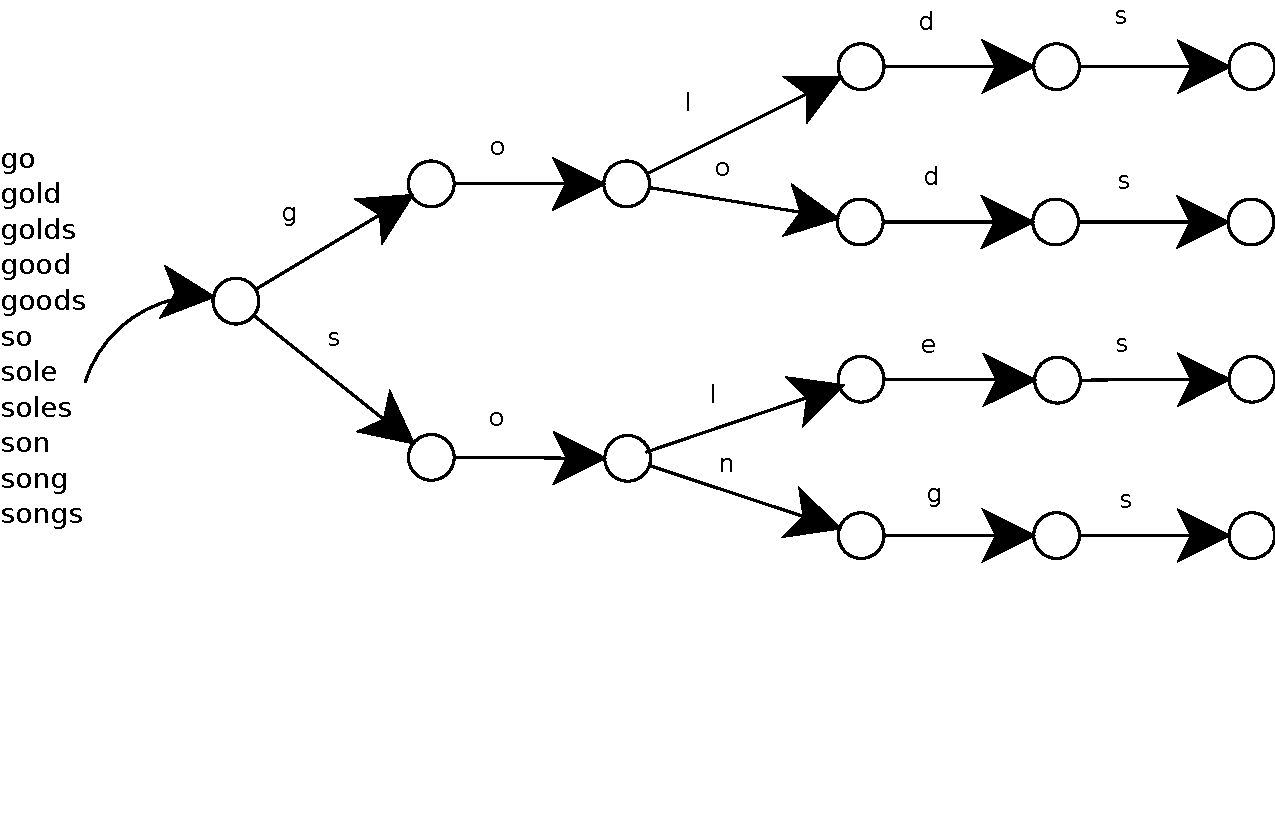
\includegraphics[scale=1]{trie}
\caption{Example of a trie data structure representing a small dictionary consisting of 11 words represented with a trie data structure. End of words is marked with grey nodes.}
\label{fig:trie}
\end{figure}

Appel and Jacobsen showed that the size of the dictionary representation can be reduced with a \emph{Directed Acyclic Word Graph}, referred to as a \emph{DAWG} \cite{fastest}. The DAWG can be constructed by first creating a trie and minimizing it by finding cases where two or more words can share a common letter (node). A new edge is then created from the previous node in one of the words to the other words node. Finally, the unnecessary edge and node are removed. See figure \ref{fig:dawg}.

A trie has a lot of redundancy, because identical edges and nodes are stored, while the DAWG allows elimination of duplications. In the DAWG example in figure \ref{fig:dawg} on can see that there are 10 nodes and 12 edges. This is significantly less than the 17 nodes and 16 edges the same dictionary would consume in the trie in figure \ref{fig:trie}. Another example is illustrated in Appel and Jacobsen's paper\cite{fastest}. A dictionary consisting of more than 100 000 words occupies 0.5 MB with a trie, but is reduced to only 175 kB with a DAWG.

\begin{figure}[h]
\centering
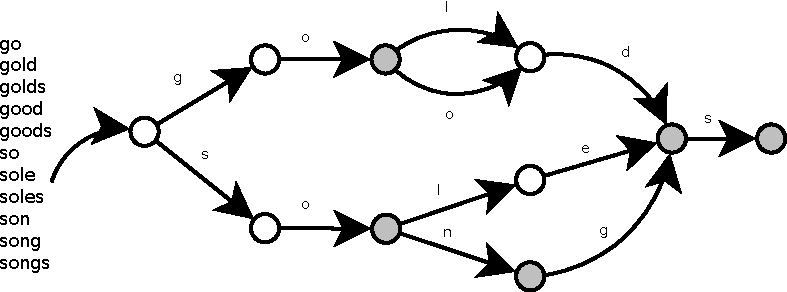
\includegraphics[scale=1]{dawg}
\caption{Example of a small dictionary consisting of 11 words represented with a DAWG. End of words marked with grey nodes.}
\label{fig:dawg}
\end{figure}

\subsection{Word generation algorithm}
\label{sec:generation}
Finding and forming words to lay out on the board is difficult. Appel and Jacobsen presented a solution to the problem by reducing the board to one dimension. Instead of searching both horizontally and vertically, it is possible to generate words only horizontally. The argument is that generating a word vertically is basically the same thing, with the only difference that the board is transposed. Therefore, the word generation algorithm is limited to only find words horizontally. Two searches are made for each move, and one of them over the transposed board. \cite{fastest}


\subsubsection{Anchor squares}
\label{sec:anchors}
A key in the algorithm implemented is the concept of \emph{anchor squares}. Anchor squares are empty squares adjacent to the words placed on the board, as can be seen in the figure \ref{fig:anchors}. These are important since words can only be extended from already existing tiles. In the first move of the game there is only one anchor; the center square, since the word in the first turn always has to be placed over the center square.

\begin{figure}[h]
\centering
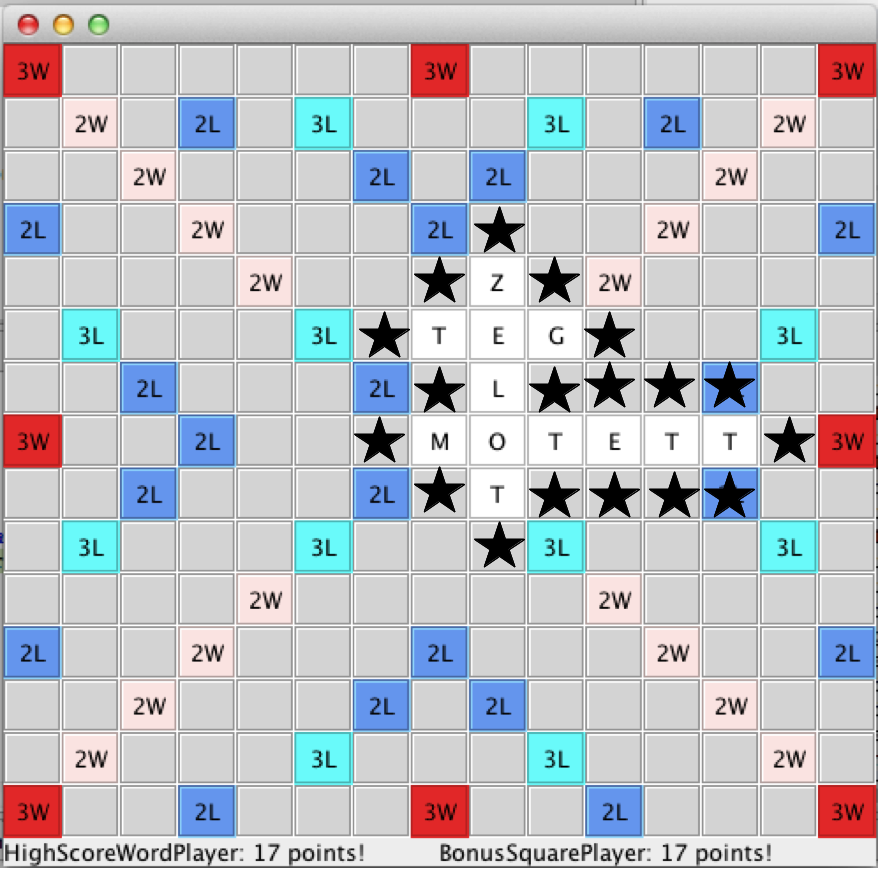
\includegraphics[scale=0.3]{anchors}
\caption{Anchor squares. The adjacent tiles are the anchor tiles from which the word generation begins.}
\label{fig:anchors}
\end{figure}

\subsubsection{Cross-checks}
\label{sec:crosscheck}
The set of available legal letters for one square is in Appel and Jacobsen's paper \cite{fastest} referred to as a \emph{cross-check set}. When placing a word horizontally, the vertically placed letters also have to form a legal word. It is quite easy to establish that if a word is placed horizontally, the vertical word can increase with only one letter at a time. This makes it possible to calculate, for each anchor square, which set of letters that are possible to place at that square. The calculations can be made before each move, and allows the algorithm to place a word by row, without considering the rest of the board. 

\subsection{Game strategies}
\label{sec:strategies}
Some of the different Scrabble game strategies is:

\begin{itemize}
\item {\bf Difficult letters}: letters with high score are usually more difficult to place and should be used as soon as possible e.g. Z or C.
\item {\bf Balance on the rack}: it is easy to get stuck with only consonants or only vowels on the rack. Keeping a good balance can be a good idea to help construct words in the next turn.
\item {\bf Bonus squares}: hitting the bonus squares will generate a higher score. It is also important to occupy them first to destroy the bonus opportunities for the opponent.
\item {\bf Word extensions}: the ability to identify extensions (i.e. prefixes and suffixes) to words, is a key to being a successful player. Such moves can generate very high scores, as the word will use many existing tiles \cite{perfectgame}.
\item {\bf Vocabulary}: there are many short words in the language, and it is rewarding if a player can learn many short word letters whic are easy to lay out.
\end{itemize}





\chapter{Implementation}
The study is based on an implementation of the word generator algorithm that follows the example of Appel and Jacobsen \cite{fastest}. Since the aim of the study is to test game strategies and not optimize disk space (as shown in \ref{dic-rep}), a DAWG seemed like a time consuming project and the choice was made to use a trie.

A slight limitation of the game rules and play were made in the implementation to make the work load fit into the given time span. The game limitations are described in section \ref{sec:limitations}.

Three different agents were implemented with different strategies to follow and they are all described in section \ref{sec:agents}.

\section{Limitations}
\label{sec:limitations}
Almost all tournament play involve only two players. The tests is therefore run with two agents. There exists a large variation of the game rules. The rules used in the study are slightly simplified versions of the most common rules used by clubs and tournament play worldwide \cite{forbund} \cite{ABSP} \cite{NASPA}.

The game is limited to be played by only two players, and the implementation is customized to not handle more players. The players have two options during a turn; either lay a word, or pass the turn and receieve zero points. In other words; the possibility to change tiles if no word can be found is removed. 

The bag is minimized, and do not contain any blank tiles or other special tiles. The result is that Q and W can never be used. The allowed tiles can be seen in the list in section \ref{letter+table}. Additionally, the agents play the game with a Swedish dictionary; Den Stora Svenska Ordlistan \cite{dictionary}.

\section{Agents}
\label{sec:agents}
To see which of the very basic strategies listed in section \ref{sec:strategies} is the most successful one against the others, three agents with different strategies were implemented. They will play against each other in order to generate results for later analyze. This section describes the three different agents implemented, and their strategy in the game. In order to evaluate which strategies are the more rewarding, the agents are each implemented with only \emph{one} strategy. The agents will be referred to as the HSW player, the BS player and the BOR player (see section \ref{sec:terminology}).

\subsection{High Score Word player}
One strategy to follow when playing Scrabble is to exploit the fact that som letters are worth more than others. These letter are less frequent in the Swedish language and therefore more difficult to use. Naturally, one would want to use them as soon as there is an opportunity, to not risk difficult situations later in the game. The HSW player prefers placing words including high score letters. By all legal moves generated, the HSW player will choose the one where the word itself has the highest score. The HSW algorithm is as follows:

\begin{lstlisting}
function ChooseMove(inputMove)
	if score of inputMove.word  > highestScore
		nextMove <- inputMove;
	end if
end function
\end{lstlisting}

The HSW player saves one move. If a better move is found than the one saved, the new move will overwrite the old one.

\subsection{Bonus Square player}
Sometimes, it can be more rewarding to place a relatively short word than a longer one. This is because of the bonus squares. They can multiply the value of either one letter, or the entire word placed, and can therefore generate high scores. The second agent strives to place words over bonus squares. If there is an opportunity to reach several bonus squares, the most rewarding bonus square is chosen depending on what word or letter is placed on the bonus. The algorithm is as follows:

\begin{lstlisting}
function ChooseMove(inputMove)
	bonus <- 0;
	for each letter in inputMove.word
		squareBonus <- bonus for letter.square;
		if squareBonus greater than bonus
			bonus <- squareBonus;
		end if 
	end for
	
	if bonus is higher than highestBonus
		nextMove <- inputMove;
		highestBonus <- bonus;
	end if
end function
			
\end{lstlisting}

\subsection{Balance On Rack player}
An important thing to think about when playing Scrabble is to plan for the next move. If a player ends up with only consonants on the rack, the possibility of laying out a word is reduced. The third agent tries to always keep a good balance between vowels and consonants on the rack, to help out form words in the next turn. The agent knows the \emph{ideal ratio} and tries to lay out words so that the tiles left on rack after a move returns a ratio as close to the ideal ratio as possible. Tests with different ideal ratios are made and the algorithm is shown below.

\begin{lstlisting}

function ChooseMove(inputMove)
	ratio <- number of vowels on rack / 
				number of tiles on rack;

	difference <- abs(ratio - idealRatio);

	if difference is less than ratioDifference
		nextMove <- inputMove;
		ratioDifference <- difference;
	end if
end function
\end{lstlisting}

\chapter{Results}
\label{sec:analysis}
Each of the agents has been tested against the others, to allow evaluation of the impact of each strategy. Explanations of the agents can be read about in section \ref{sec:agents}. 

Section \ref{sec:conditions} describes under which conditions the tests were made.

Sections \ref{sec:highBalance}, \ref{sec:balanceBonus} and \ref{sec:bonusHigh} show the results from each run.
 
\section{Test conditions}
The BOR player has an ideal ratio between the tiles on the rack which it tries to keep throughout the game. The ratio will be referred to as the \emph{vowel ratio} and is defined as the number of vowels divided in the total number of tiles on the rack.

\label{sec:conditions}
\subsection{Games}
In one run the agents were set to play 1000 games against each other and to minimize the impact of opening the game in the results, both agents started the game 500 times. Each run were made 10 times, so the total result is based on 10 000 games. It was established that there were no significant changes in the results between running 1000 games, and 10 000 games, and would therefore probably be reduntant to make more tests. The decision to run 1000 games at a time were due to an unknown bug causing the word generation algorithm to run very slow after approximately 1800 games.

\subsection{Dictionaries}

The tests are based on two variations of the Swedish dictionary. The first is the small dictionary, which consists of the words only in their base form in the Swedish dictionary. Ths size of the small dictionary is 83247 words. The second is the large dictionary, which includes all possible inflections of each word making it as large as 480 391 words.

The rules of the English Scrabble allow the players to form inflections. However, the Swedish rules do not. It seemed interesting to compare the results from using both the large dictionary the small. The dictionary available could be especially relevant for the results of the BS player. It makes use of the bonus squares, which could be easier to reach with short word extensions if all words are allowed.


\section{High score words vs Balance On Rack}
\label{sec:highBalance}

Several tests were made with the BOR player, using different values for the vowel ratio. From table \ref{tab:bor+hsw} one can even in the best best case for the BOR player, it only wins 12\% of the games. Note that there is a significant peak in the number of winnings when the ratio is set to 8/8, and also an extreme bottom when the ratio is set to 1/8.


\begin{table}[h]
\centering
    \begin{tabular}{ c | c | c p{5cm}}
   	Vowel ratio & HSW wins & BOR wins \\ \hline
	0/8 & 9922 & 73 \\ 
    	1/8 & 9999  & 1 \\ 
    	2/8 & 9484 & 507 \\
    	3/8 & 9777 & 212 \\
	4/8 & 9735 & 262 \\ 
	5/8 & 9627 & 368 \\ 
	6/8 & 9146 & 838 \\ 
	7/8 & 9863 & 134 \\ 
	8/8 & 8762 & 1206 \\
    \end{tabular}
\caption{Winnings over 10000 games depending on vowel ratio. The ratio is defined by the number of vowels divided by the number of tiles on rack.}
\label{tab:bor+hsw}
\end{table}


The HSW player is a more successful player, with a winning percentage of at least 88\%. As one can see in table \ref{tab:borhswstats8} and table \ref{tab:borhswstats8smallDict} in the appendix, both players won slightly more games when starting the game. The HSW player had an average of 50.5\% of the winnings after starting the game, and the BOR player had 52.3\%. 


Another observation is that the BOR player is not as affected by the size of the dictionary as the HSW player. The BOR player wins 53\% more games with the small dictionary compared to the large. The HSW player, however, wins 8\% more games with the large dictionary than with the small. The results from 10 000 games can be seen in figure \ref{fig:highBalanceBothDict}.

\graphicspath{{../results/Plots/}}

\begin{figure}[h]
\centering
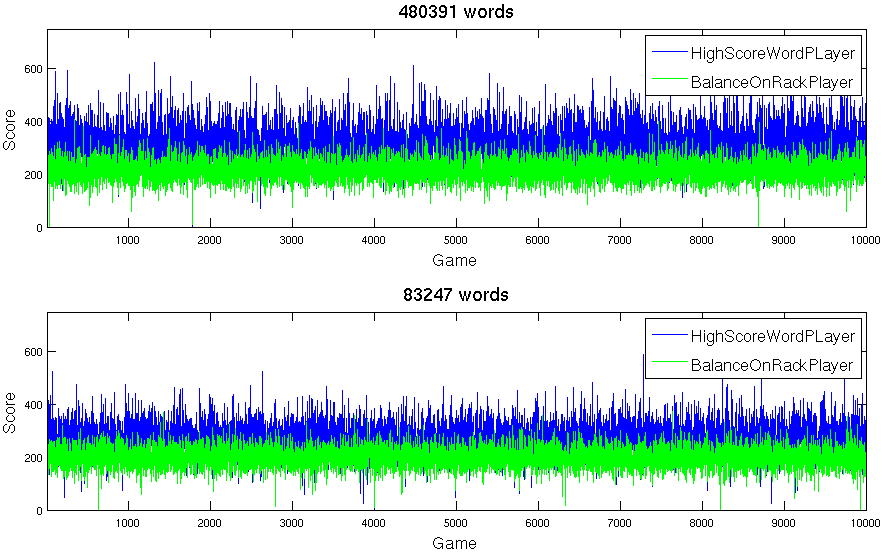
\includegraphics[scale=0.4]{HighBalance8vow_bothDict_cropped}
\caption {Scores with a BOR vowel ratio 8/8. The game scores from the HSW player and BOR player in 10000 games}
\label{fig:highBalanceBothDict}
\end{figure}




\section{Balance On Rack vs Bonus Squares}
\label{sec:balanceBonus}
The BOR player shows a poor performance also against the BS player, with a best case of 9\% winnings. Table \ref{tab:bor+bs} shows that the vowel ratio of 8/8 gives a much better result for the BOR player than any other vowel ratio, although it is still outnumbered by the BS player.

\begin{table}[h]
\centering
    \begin{tabular}{ c | c | c  p{5cm}}
   	Vowel ratio & BS wins & BOR wins \\ \hline
	0/8 & 9925 & 72 \\ 
    	1/8 & 9987 & 12 \\ 
    	2/8 & 9670 & 325 \\ 
    	3/8 & 9829 & 165 \\ 
	4/8 & 9818 & 172 \\ 
	5/8 & 9731 & 261 \\ 
	6/8 & 9370 & 620 \\ 
	7/8 & 9859 & 141 \\ 
	8/8 & 9074 & 915 \\ 
    \end{tabular}
\caption{Winnings over 10000 games depending on vowel ratio. The ratio is defined by the number of vowels divided by the number of tiles on rack.}
\label{tab:bor+bs}
\end{table}

Of all winnings made by the BS player, 51\% were achieved after being the starting player. For the BOR player the percentage is 54\%. This can be seen in table \ref{tab:borbsstats8} and table \ref{tab:borbsstats8smallDict} in the appendix. One can also see that the first move has a more significant impact on the BOR player's results. The BS player, however, seems to be able to compensate a possible loss, when not starting, later in the game.

As in the previous section, the BOR player is not as affected by the size of the dictionary as the BS player. In figure \ref{fig:bonusBalanceLargeDict} one can see that the BS player is performing significantly better with a larger dictionary. The number of winnings is increased by 11\% when enabling the large dictionary. The BOR player on the other hand almost doubles the number of winnings when only the small dictionary is available with a winning rate increase of 97\%. 



\begin{figure}[h]
\centering
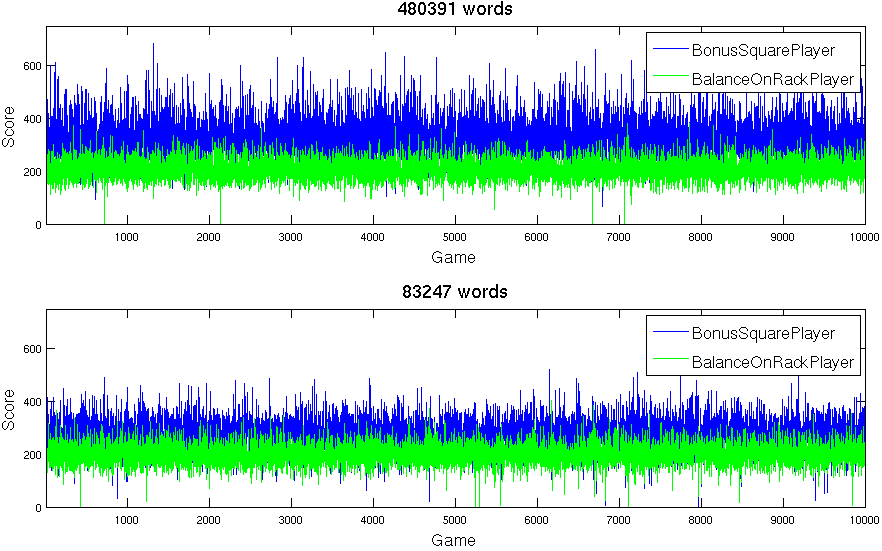
\includegraphics[scale=0.4]{BonusBalance8vow_bothDict_cropped}
\caption {Scores with vowel ratio 8/8. Scores of the two players in 1000 games with 480 391 words available.}
\label{fig:bonusBalanceLargeDict}
\end{figure}



\section{Bonus Squares vs High Score Words}
\label{sec:bonusHigh}
The BS player wins just over 6 of 10 times against the HSW player when using all inflection forms from the Swedish dictionary table \ref{table:bs+hsw+allwords} and well over 5 of 10 times when only the base forms of words is used table \ref{table:bs+hsw+baseforms}. When the BS player started playing it won 52\% of its wins when using all inflection forms. For the HSW player 53\% of its wins. When using only the base form both of them were winning 51\% its wins when started laying out words.

\begin{table}[h]
\centering
    \begin{tabular}{ l | c | c }
   	& Bonus Squares & High score words \\
   	\hline
   	Wins & 6104 & 3857 \\
   	Draws & 39 & 39 \\   	
	Wins when started playing & 3148 & 2040 \\   	
	Mean score & 308 & 278 \\
	Median score & 301 & 273 \\	 	 
	Highest score & 724 & 606 \\
	Lowest score & 85 & 61 \\		
    \end{tabular}
\caption{Result from 10 000 games with words in all inflection forms from the Swedish dictionary (480 391 words).}
\label{table:bs+hsw+allwords}
\end{table}

\begin{table}[h]
\centering
    \begin{tabular}{ l | c | c }
   	& Bonus Squares & High score words \\
   	\hline
   	Wins & 5427 & 4521 \\
   	Draws & 52 & 52 \\
	Wins when started playing & 2758 & 2314 \\   	
	Mean score & 248 & 240 \\
	Median score & 246 & 234 \\	 	 
	Highest score & 488 & 506 \\
	Lowest score & -15 & -11 \\		
    \end{tabular}
\caption{Result from 10 000 games with words in base form from the Swedish dictionary (83 247 words).}
\label{table:bs+hsw+baseforms}
\end{table}

The resulting mean, median, highest and lowest scores are significantly higher when using all inflection forms. Lowest score is negative for both players when using only base forms. The BS player's mean score is 24\% higher in table \ref{table:bs+hsw+allwords} compared to table \ref{table:bs+hsw+baseforms}. The same applies for the end score which is higher when using all words, which can be seen in figure \ref{fig:bs+hsw+totalscores}.

\begin{figure}[h]
\centering
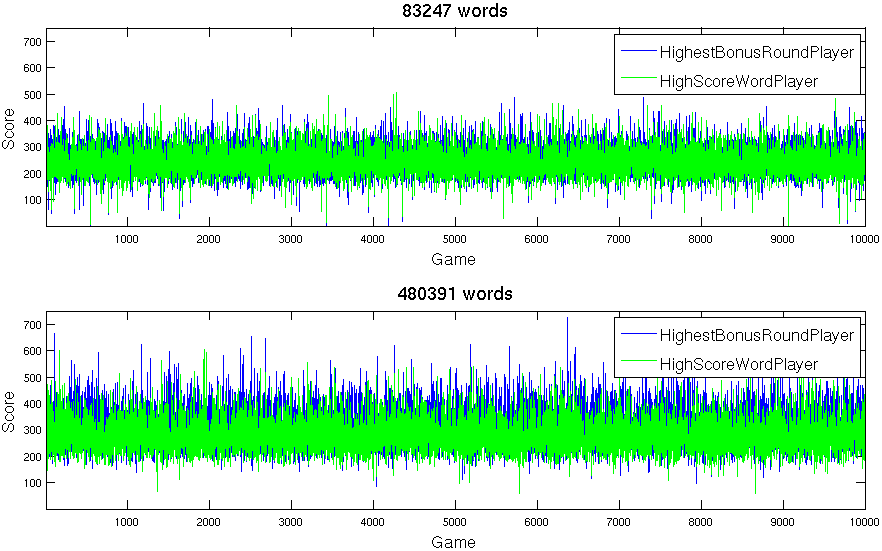
\includegraphics[scale=0.4]{Highest_Bonus_Round_vs_High_Score_Word_10000_cropped}
\caption {End scores of the two players in 10000 games. Upper graph with base words only and lower graph with all inflection forms.}
\label{fig:bs+hsw+totalscores}
\end{figure}



\chapter{Conclusions}
\section{Discussions}
The reason for the negative scores can be due to an impossible situation from the start. The agents were for example given only consonants that cannot form a word, or only difficult tiles. This would result a situation where none of the players being able to place a word, and the game eventually ends. The sum of the letter scores on the rack is then subtracted, and it is the only way a player could get a negative score.

\subsubsection{BOR player}
The BOR player is significantly better with a vowel ratio of 8/8. It can probably be explained from the fact that when choosing a move, and the vowel ratio is 8/8 (1) it is easier for the agent to place longer words. Imagine the agent placing a word using all tiles but one, and the remaining tile on hand is a vowel. This would be a preferable move if the ratio is 1, but not if the ratio is less. If the ratio would be 4/8 for example, the agent would choose a move that leaves two tiles, where one is a vowel, over the move with a longer word. 

There is however a hole in the theory. The phenomena that occurs with a vowel ratio of 7/8; the extremely bad winning rate. After speculating and trying to explain this occurence, we are still stunned. If the theory of allowing longer words with a higher ratio would be correct, the result ought to increase with the vowel ratio.

\subsubsection{HSW player}
The HSW player is on the same level as the BS player when it comes to mean score over the games. However, the reason for playing as good could be that the BS player probably hits the bonuses and generates very high scores at times. As seen in the tables in section \ref{sec:tablesbs}, the BS player has a significantly higher maximum score than the HSW player.

\subsubsection{BS player}
Choosing to place words that will occupy a bonus square is rewarding. It will not only give a high score but will also destroy the possiblity for the opponent to reach a bonus square.

It has active playing style with the mission to conquer the bonus squares at all cost. With the power of a big dictionary it will have a higher probability to reach a bonus. It is easy to extend words already on board when having the possibility to use all inflection forms of words. The end score will also be higher Figure \ref{fig:bs+hsw+totalscores}. When using only base words it will struggle to find bonus squares. This is due to //TODO

\subsubsection{Moreover}
This study is very limited, which can affect the results. One should not consider these player as superior, or even equal, to a human player. The objective was to examine different strategies separately, and most human players use several strategies simultaneously \cite{perfectgame}. The agents tested in this study were implemented with only one strategy, and an agent who calculates the total score of a move and chooses the highest one wuld probably win without effort over all three tested agents. 

\section{Conclusions}
Some conclusion made from the results is that it seems to be of advantage to start the game, although a slight one. All result show that of the winning games, a little over 50\% were made when the player had started the game.

Bonus squares are more important than one maybe imagines. It is not always the best move to place a long word with the highest score, since the bonus squares, if used wisely, can generate extremely high scores. Use of difficult letters together with the bonus squares is probably an intelligent approach.

To keep the balance on the rack is useless, if no scores are taken into consideration. One could for instance generate as high score words as possible, together with keeping the balance.

subsection{Future work}
If there is interest, this work can be extended in many ways. One can for instance try and implement other types of agents. For this study there were reflections about implementing agents that calculates the score from a move and get penalty points for moves less preferable according to the strategy. 

\appendix
\chapter{Tables}

\section{High Score Words vs Balance On Rack}
\subsection{Small dictionary (83 247 words)}
\begin{table}[h]
\centering
    \begin{tabular}{ l | l | l }
   	& BOR & HSW \\
   	\hline
   	Wins & 1850 & 8114 \\
	Draws & 36 & 36 \\
	Wins when started playing & 950 & 4088 \\   	
	Mean score & 198 & 263 \\
	Median score & 199 & 262\\	 	 
	Highest score & 373 & 590 \\
	Lowest score & -17 & -13 \\		
    \end{tabular}
\caption{Result from 10 000 games with vowel ratio 8/8 and words in base form from the Swedish dictionary (83 247 words).}
\label{tab:borhswstats8smallDict}
\end{table}

\subsection{Large dictionary (480 391 words)}
\begin{table}[h]
\centering
    \begin{tabular}{ l | l | l }
   	& BOR & HSW \\
   	\hline
   	Wins & 1206 & 8762 \\
	Draws & 32 & 32 \\
	Wins when started playing & 643 & 4431 \\   	
	Mean score & 214 & 309 \\
	Median score & 213 & 307 \\	 	 
	Highest score & 407 & 624 \\
	Lowest score & -9 & -19 \\		
    \end{tabular}
\caption{Result from 10 000 games with vowel ratio 8/8 and words in all inflection forms from the Swedish dictionary (480 391 words).}
\label{tab:borhswstats8}
\end{table}

\begin{table}[h]
\centering
    \begin{tabular}{ l | l | l }
   	& BOR & HSW \\
   	\hline
   	Wins & 134 & 9863 \\
	Draws & 3  & 3 \\
	Wins when started playing & 69 & 4943 \\   	
	Mean score & 163 & 374 \\
	Median score & 161 & 372 \\	 	 
	Highest score & 371 & 774 \\
	Lowest score & -20 & -13 \\		
    \end{tabular}
\caption{Result from 10 000 games with vowel ratio 7/8 and words in all inflection forms from the Swedish dictionary (480 391 words).}
\label{tab:borhswstats7}
\end{table}

\begin{table}[h]
\centering
    \begin{tabular}{ l | l | l }
   	& BOR & HSW \\
   	\hline
   	Wins & 838 & 9146 \\
	Draws & 16  & 16 \\
	Wins when started playing & 464 & 4629 \\   	
	Mean score & 203 & 309 \\
	Median score & 202 & 307 \\	 	 
	Highest score & 362 & 676\\
	Lowest score & 74 & 97 \\		
    \end{tabular}
\caption{Result from 10 000 games with vowel ratio 6/8 and words in all inflection forms from the Swedish dictionary (480 391 words).}
\label{tab:borhswstats6}
\end{table}

\begin{table}[h]
\centering
    \begin{tabular}{ l | l | l }
   	& BOR & HSW \\
   	\hline
   	Wins & 368 & 9627 \\
	Draws & 5 & 5 \\
	Wins when started playing & 176 & 4815 \\   	
	Mean score & 190 & 322 \\
	Median score & 190 & 318 \\	 	 
	Highest score & 346 & 672 \\
	Lowest score & -17 & -18\\		
    \end{tabular}
\caption{Result from 10 000 games with vowel ratio 5/8 and words in all inflection forms from the Swedish dictionary (480 391 words).}
\label{tab:borhswstats5}
\end{table}

\begin{table}[h]
\centering
    \begin{tabular}{ l | l | l }
   	& BOR & HSW \\
   	\hline
   	Wins & 262 & 9735 \\
	Draws & 3 & 3 \\
	Wins when started playing & 142 & 4890 \\   	
	Mean score & 189 & 336  \\
	Median score & 188 & 333 \\	 	 
	Highest score & 329 & 657 \\
	Lowest score & -24 & -21\\		
    \end{tabular}
\caption{Result from 10 000 games with vowel ratio 4/8 and words in all inflection forms from the Swedish dictionary (480 391 words).}
\label{tab:borhswstats4}
\end{table}

\begin{table}[h]
\centering
    \begin{tabular}{ l | l | l }
   	& BOR & HSW \\
   	\hline
   	Wins & 212 & 9777 \\
	Draws & 11 & 11 \\
	Wins when started playing & 95 & 4889 \\   	
	Mean score & 183 & 328  \\
	Median score & 183 & 324 \\	 	 
	Highest score & 337 & 784 \\
	Lowest score & -24 & -23\\		
    \end{tabular}
\caption{Result from 10 000 games with vowel ratio 3/8 and words in all inflection forms from the Swedish dictionary (480 391 words).}
\label{tab:borhswstats3}
\end{table}

\begin{table}[h]
\centering
    \begin{tabular}{ l | l | l }
   	& BOR & HSW \\
   	\hline
   	Wins & 507 & 9484 \\
	Draws & 9 & 9 \\
	Wins when started playing & 278 & 4777 \\   	
	Mean score & 191 & 310 \\
	Median score & 190 & 306 \\	 	 
	Highest score & 347 & 676 \\
	Lowest score & -17 & -10 \\		
    \end{tabular}
\caption{Result from 10 000 games with vowel ratio 2/8 and words in all inflection forms from the Swedish dictionary (480 391 words).}
\label{tab:borhswstats2}
\end{table}

\begin{table}[h]
\centering
    \begin{tabular}{ l | l | l }
   	& BOR & HSW \\
   	\hline
   	Wins & 1 & 9999 \\
	Draws & 0 & 0 \\
	Wins when started playing & 0 & 5009 \\   	
	Mean score & 124 & 420 \\
	Median score & 123 & 415 \\	 	 
	Highest score & 299 & 745 \\
	Lowest score & -16 & -12 \\		
    \end{tabular}
\caption{Result from 10 000 games with vowel ratio 1/8 and words in all inflection forms from the Swedish dictionary (480 391 words).}
\label{tab:borhswstats1}
\end{table}

\begin{table}[h]
\centering
    \begin{tabular}{ l | l | l }
   	& BOR & HSW \\
   	\hline
   	Wins & 73 & 9922 \\
	Draws & 5 & 5 \\
	Wins when started playing & 38 & 4974 \\   	
	Mean score & 164 & 354 \\
	Median score & 164 & 350 \\	 	 
	Highest score & 357 & 716 \\
	Lowest score & -19 & -11 \\		
    \end{tabular}
\caption{Result from 10 000 games with vowel ratio 0/8 and words in all inflection forms from the Swedish dictionary (480 391 words).}
\label{tab:borhswstats0}
\end{table}

\FloatBarrier
\section{Balance On Rack vs Bonus Squares} 
\label{sec:tablesbs}
\subsection{Small dictionary (83 247 words)}

\begin{table}[h]
\centering
    \begin{tabular}{ l | l | l }
   	& BOR & BS \\
   	\hline
   	Wins & 1798 & 8165 \\
	Draws & 37 & 37 \\
	Wins when started playing & 951 & 4142 \\   	
	Mean score & 198 & 266 \\
	Median score & 198 & 264\\	 	 
	Highest score & 405 & 527 \\
	Lowest score & -23 & -17 \\		
    \end{tabular}
\caption{Result from 10 000 games with vowel ratio 8/8 and words in base form from the Swedish dictionary (83 247 words).}
\label{tab:borbsstats8smallDict}
\end{table}

\subsection{Large dictionary (480 391 words)}
\begin{table}[h]
\centering
    \begin{tabular}{ l | l | l }
   	& BOR & BS \\
   	\hline
   	Wins & 915 & 9074 \\
	Draws & 11 & 11 \\
	Wins when started playing & 496 & 4588 \\   	
	Mean score & 207 & 321 \\
	Median score & 206 & 318\\	 	 
	Highest score & 382 & 682 \\
	Lowest score & -25 & -19 \\		
    \end{tabular}
\caption{Result from 10 000 games with vowel ratio 8/8 and words in all inflection forms from the Swedish dictionary (480 391 words).}
\label{tab:borbsstats8}
\end{table}

\begin{table}[h]
\centering
    \begin{tabular}{ l | l | l }
   	& BOR & BS \\
   	\hline
   	Wins & 141 & 9859 \\
	Draws & 0 & 0 \\
	Wins when started playing & 80 & 4949 \\   	
	Mean score & 164 & 321 \\
	Median score & 162 & 378\\	 	 
	Highest score & 380 & 733 \\
	Lowest score & -14 & -17 \\		
    \end{tabular}
\caption{Result from 10 000 games with vowel ratio 7/8 and words in all inflection forms from the Swedish dictionary (480 391 words).}
\label{tab:borbsstats7}
\end{table}

\begin{table}[h]
\centering
    \begin{tabular}{ l | l | l }
   	& BOR & BS \\
   	\hline
   	Wins & 620 & 9370\\
	Draws & 10 & 10 \\
	Wins when started playing & 340 & 4725 \\   	
	Mean score & 195 & 321 \\
	Median score & 195 & 316 \\	 	 
	Highest score & 416 & 749 \\
	Lowest score & -25 & -26 \\		
    \end{tabular}
\caption{Result from 10 000 games with vowel ratio 6/8 and words in all inflection forms from the Swedish dictionary (480 391 words).}
\label{tab:borbsstats6}
\end{table}

\begin{table}[h]
\centering
    \begin{tabular}{ l | l | l }
   	& BOR & BS \\
   	\hline
   	Wins & 261 & 9731\\
	Draws & 8 & 8 \\
	Wins when started playing & 139 & 4884 \\   	
	Mean score & 185 & 336 \\
	Median score & 186 & 333 \\	 	 
	Highest score & 388 & 830 \\
	Lowest score & -14 & -19 \\		
    \end{tabular}
\caption{Result from 10 000 games with vowel ratio 5/8 and words in all inflection forms from the Swedish dictionary (480 391 words).}
\label{tab:borbsstats5}
\end{table}

\begin{table}[h]
\centering
    \begin{tabular}{ l | l | l }
   	& BOR & BS \\
   	\hline
   	Wins & 172 & 9818 \\
	Draws & 10 & 10 \\
	Wins when started playing & 97 & 4930 \\   	
	Mean score & 184 & 350 \\
	Median score & 183 & 347 \\	 	 
	Highest score & 343 & 742 \\
	Lowest score & -17 & -20 \\		
    \end{tabular}
\caption{Result from 10 000 games with vowel ratio 4/8 and words in all inflection forms from the Swedish dictionary (480 391 words).}
\label{tab:borbsstats4}
\end{table}

\begin{table}[h]
\centering
    \begin{tabular}{ l | l | l }
   	& BOR & BS \\
   	\hline
   	Wins & 165 & 9829 \\
	Draws & 6 & 6 \\
	Wins when started playing & 92 & 4935 \\   	
	Mean score & 178 & 340 \\
	Median score & 178 & 337 \\	 	 
	Highest score & 365 & 807 \\
	Lowest score & -12 & -10 \\		
    \end{tabular}
\caption{Result from 10 000 games with vowel ratio 3/8 and words in all inflection forms from the Swedish dictionary (480 391 words).}
\label{tab:borbsstats3}
\end{table}

\begin{table}[h]
\centering
    \begin{tabular}{ l | l | l }
   	& BOR & BS \\
   	\hline
   	Wins & 325 & 9670 \\
	Draws & 5 & 5 \\
	Wins when started playing & 168 & 4851 \\   	
	Mean score & 184 & 323 \\
	Median score & 184 & 319 \\	 	 
	Highest score & 360 & 668 \\
	Lowest score & -20 & -24 \\		
    \end{tabular}
\caption{Result from 10 000 games with vowel ratio 2/8 and words in all inflection forms from the Swedish dictionary (480 391 words).}
\label{tab:borbsstats2}
\end{table}

\begin{table}[h]
\centering
    \begin{tabular}{ l | l | l }
   	& BOR & BS \\
   	\hline
   	Wins & 12 & 9987 \\
	Draws & 1 & 1 \\
	Wins when started playing & 3 & 5000 \\   	
	Mean score & 126 & 428 \\
	Median score & 126 & 426 \\	 	 
	Highest score & 324 & 801 \\
	Lowest score & -19 & -16 \\		
    \end{tabular}
\caption{Result from 10 000 games with vowel ratio 1/8 and words in all inflection forms from the Swedish dictionary (480 391 words).}
\label{tab:borbsstats1}
\end{table}

\begin{table}[h]
\centering
    \begin{tabular}{ l | l | l }
   	& BOR & BS \\
   	\hline
   	Wins & 72 & 9925 \\
	Draws & 3 & 3 \\
	Wins when started playing & 41 & 4976 \\   	
	Mean score & 162 & 369 \\
	Median score & 161 & 367 \\	 	 
	Highest score & 316 & 838 \\
	Lowest score & -11 & -21 \\		
    \end{tabular}
\caption{Result from 10 000 games with vowel ratio 0/8 and words in all inflection forms from the Swedish dictionary (480 391 words).}
\label{tab:borbsstats0}
\end{table}

\begin{thebibliography}{100}  
  \bibitem{perfectgame} Sheppard, B., 2002, Towards Perfect Play of Scrabble, Maastricht.
  \bibitem{fastest} Appel A. W., Jacobson, G. J., 1985, The World’s Fastest Scrabble Program, Commun. ACM, 31(5), 572-585, May 1988.
\bibitem{faster} Gordon, S. A., 1993, A Faster Scrabble Move Generation Algorithm, Software - Practice and experience, Vol. 24(2), 219-232, February 1994.
\bibitem{ai} Russell S., Norvig P. Artificial Intelligence: A Modern Approach 3rd ed. Prentice Hall. 2009
\bibitem{inforetrieve} Manning C. D., Raghavan P., Schütze H., Introduction to Information Retrieval, Cambridge University Press, 2008, p. 49-65.
\bibitem{dictionary} Den stora svenska ordlistan (Swedish dictionary), http://code.google.com/p/dsso/downloads/detail?name=dsso-1.52.txt\&can=1\&q=
\bibitem{forbund} Swedish tournament rules by Svenska Scrabbleförbundets, http://www.scrabbleforbundet.se/index.php?option=content\&task=view\&id=16\&Itemid=39
\bibitem{ABSP} World English-Language Scrabble Players’ Association (WESPA) rules, http://www.wespa.org/rules/RulesV2nov11.pdf
\bibitem{NASPA} North American SCRABBLE Players Association official tournament rules, http://www.scrabbleplayers.org/wiki/images/a/af/Rules-20110605.pdf
\bibitem{letterpoints} http://en.wikipedia.org/wiki/Scrabble\_letter\_distributions
\end{thebibliography}
\end{document}